\documentclass{article}
\usepackage{enumerate}
\usepackage[margin=0.8in]{geometry}
\usepackage{hyperref}
\usepackage{graphicx}
\graphicspath{ {userStudyImgs/} }
\begin{document}

\title{PurlPal User Study Plan}
\author{Laura Eckman}
\maketitle

\section{Study Design}

\subsection{Participants}

Participants will be recruited from various knitting circles around campus.
Recruited participants must be able to knit in the ``Continental'' style, but do not need to prefer or normally use that style.

\subsection{Pre-Experiment}

Participants will sign a consent form (\ref{consent}) and fill out an informational form (\ref{participant-info}) about their existing knitting skills and preferences.
This data will be anonymous and used to provide more context to the empirically gathered data detailed in the next section.

\subsection{Experiment}

Two patterns will be involved in this experiment.
Pattern A will be 4 rows of 10 stitches each where the 3rd and 7th stitches form a stockinette column.
Pattern B will be 4 rows of 10 stitches each where the first two and last two stitches form a garter border.
Both patterns will be knitted in worsted weight yarn on size 8 straight needles.
Participants will not need to cast on - 8 rows of the same pattern will already be started for them.

Participants will start with pattern A or pattern B with equal probability to counterbalance any effects of an unintentionally ``harder'' pattern.
Since there will not be enough participants to counterbalance two variables, all participants will knit with a non-responsive electronic pattern first, then knit with PurlPal.
If significantly more participants can be recruited, participants will start with the non-responsive electronic pattern or PurlPal with equal probability.

For both conditions, the researcher will note the number of changes in visual attention from looking at the screen to looking at their knitting.
The researcher will also note how many times the participant makes a mistake and goes back to correct it.
Furthermore, the researcher will time the participants from their first completed stitch until they finish the section or start knitting.

The researcher will also record any difficulty participants have in utilizing certain functionality in PurlPal or any instances when undesired behavior is accidentally produced.

All participants will be asked to knit in the ``Continental'' style - holding their yarn in the left hand and picking it up with the needle.

\subsubsection{Condition 1: Knitting with Electronic Pattern}

Study participants will see a charted pattern displayed exactly the same way as in PurlPal, but without any row/stitch highlighting or navigational ability. See \ref{nonresponsive} for an example.

\subsubsection{Condition 2: Knitting with PurlPal}

Study participants will be read a scripted introduction (\ref{script}) to the features of PurlPal.
They will be told to hold their knitting as if to start, and the researcher will run the calibration process, wait 3 seconds, and tell the knitters to begin. See \ref{responsive} for an example.

\subsection{Post-Experiment}

Participants will fill out a qualitative evaluation of PurlPal (\ref{questionnaire}).
If time permits, participants will be able to ask questions of the researcher and provide more feedback verbally - this feedback will be captured via recording and integrated with the general feedback on the written survey.

\section{Evaluation}

Participants will be grouped into two categories:
\textbf{expert knitters}, who have been knitting for 6+ months or at least one month but have also learned every skill listed,
and \textbf{novice knitters}, who have been knitting for less than 6 months or who have not learned to either increase or decrease.

All of the following metrics will be calculated for the entire set of participants, the subset of expert knitters, and the subset of novice knitters across both experimental conditions:
\begin{itemize}
  \item Mean \& median number of times looking at pattern
  \item Mean \& median percent of time looking at pattern (for participants who allowed video recording)
  \item Mean \& median number of times looking at knitting
  \item Mean \& median percent of time looking at knitting (for participants who allowed video recording)
  \item Mean \& median number of mistakes
  \item Mean \& median total time to finish knitting
\end{itemize}

\section{Appendix}

\subsection{Participant Consent} \label{consent}

\fbox{%
  \parbox{\textwidth}{%

    Thank you for your interest in the PurlPal user evaluations!

    \medskip

    During today's experiment, you will knit under two different conditions, then fill out a feedback survey.
    The experiment should take no longer than 20 minutes.
    Note that I am testing the usability of PurlPal - not your knitting ability.
    Your answers will be confidential. If you additionally consent to be recorded, all records will be deleted as soon as the data has been processed (within 1 week of recording).
    Anonymized data will be retained for up to 1 year.

    \medskip

    Taking part in this study is completely voluntary. You may skip any questions that you do not want to answer. If you decide not to take part or to skip some of the questions, there will be no consequences.
    If you decide to take part, you are free to withdraw at any time.

    \medskip

    If you have questions: The researcher conducting this study is Laura Eckman. Please ask any questions you have now. If you have questions later, you may contact the researcher at leckman@mit.edu or at 973-558-4076.

    \medskip

    You will be given a copy of this form to keep for your records.

    \medskip

    \textbf{Statement of Consent:} \\ I have read the above information, and have received answers to any questions I asked. I consent to take part in the study.

    \medskip

    \qquad Your Name (printed):

    \qquad Your Signature:

    \qquad Date:


    \medskip

    In addition to agreeing to participate, I also consent to having the experiment video-recorded.

    \medskip

    \qquad Your Signature:

    \qquad Date:
  }%
}

\subsection{Participant Information} \label{participant-info}

\fbox{%
  \parbox{\textwidth}{%
    \textbf{Participant Information}
    \begin{enumerate}
      \item I have been knitting for: \\ \\
      $<$ 1 Month \qquad 1-6 Months \qquad 6 months - 2 years \qquad 2-5 Years \qquad 5+ years
      \item I normally knit:
        \begin{itemize}
          \item Holding the yarn in my left hand and picking it up with the right needle
          \item Holding the yarn in my right hand and wrapping it around the right needle
          \item Other:
        \end{itemize}
      \item I know how to:
        \begin{itemize}
          \item Knit
          \item Purl
          \item Cast On
          \item Bind Off
          \item Increase (yarn over, M1, etc)
          \item Decrease (k2tog, ssk, etc)
        \end{itemize}
      \item In general, I prefer knitting from electronic patterns more than from printed patterns. \\ \\
      Very True \qquad Mostly True \qquad Neutral \qquad Mostly False \qquad Very False
      \item In general, I prefer knitting from charted patterns more than from written patterns. \\ \\
      Very True \qquad Mostly True \qquad Neutral \qquad Mostly False \qquad Very False
    \end{enumerate}
  }%
}

\subsection{Experimental Interfaces}

\subsubsection{Electronic Pattern} \label{nonresponsive}

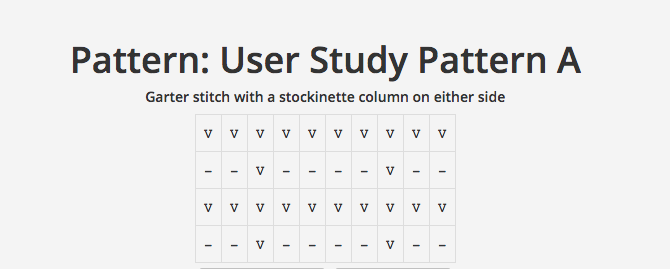
\includegraphics[width=5in]{nonresponsive_pattern_A}

\clearpage

\subsubsection{PurlPal}

\qquad \textbf{Description of Interface - Script} \label{script}

\medskip

\fbox{%
  \parbox{\textwidth}{%

  \medskip
    This is PurlPal!

    \medskip

    PurlPal will track your knitting as you move through the pattern using this sensor.
    The sensor isn't perfect, so you can also navigate through the pattern by using voice commands like ``move forward'' to go to the next stitch or ``next row'' to move to the beginning of the next row.
    You can also use these buttons or double click on any stitch to jump anywhere in the pattern.

    \medskip

    By default, PurlPal shows a chart of how the pattern looks from the right side.
    You are also welcome to look at the chart from the wrong side, or toggle between the right side and wrong side as you knit, by using these buttons.

    \medskip

    If you want to turn off motion detection or voice recognition, or you want to see available voice commands, you can find those in the settings menu here.

    \medskip

    Please get into position to start knitting so I can calibrate the sensor - but don't actually start yet.
    \\ ** calibrate sensor *
    \\ Okay, you can begin now. \medskip

  }%
}

\medskip

\textbf{Interface Example} \label{responsive}

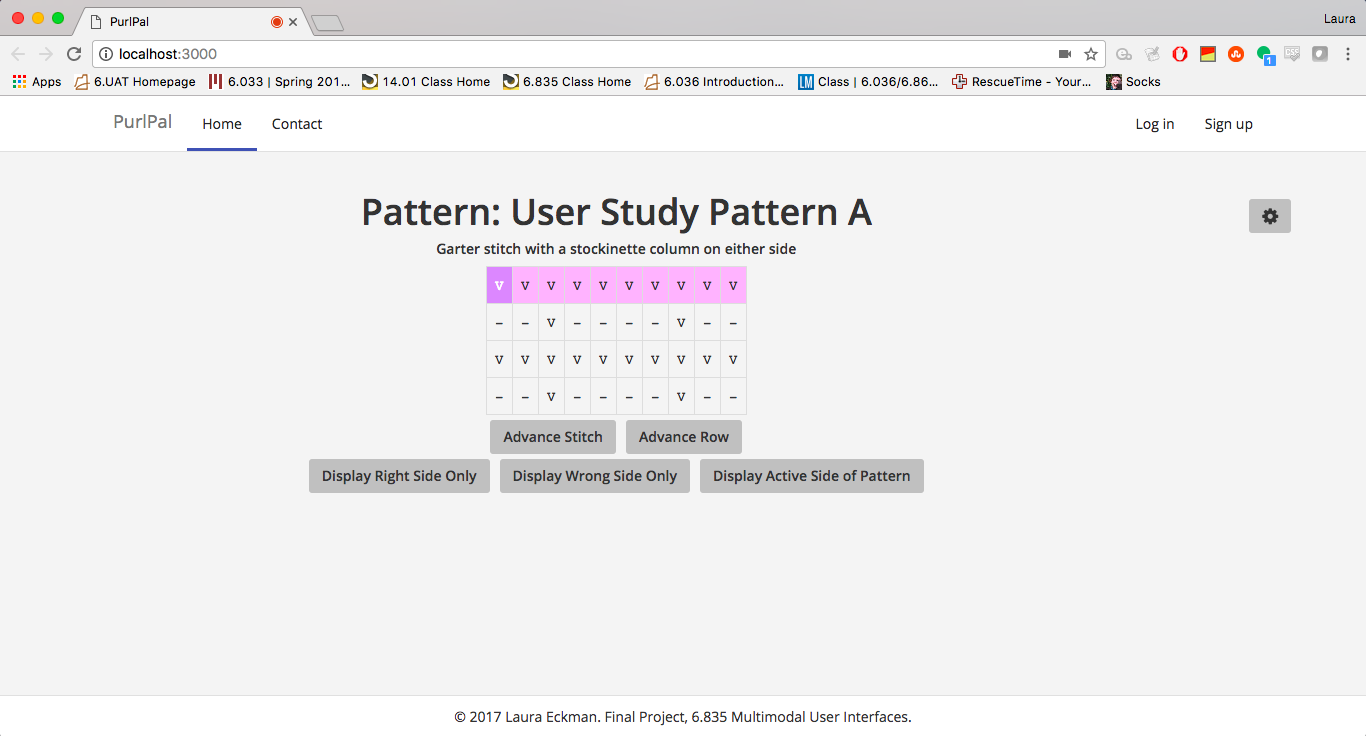
\includegraphics[width=6in]{responsive_pattern_A}

\subsection{PurlPal Questionnaire} \label{questionnaire}

\fbox{%
  \parbox{\textwidth}{%
    %\begin{center}
    \begin{enumerate}
      \item I found PurlPal easy to use. \\ \\
      Very True \qquad Mostly True \qquad Neutral \qquad Mostly False \qquad Very False
      \item I preferred navigating with speech rather than my mouse. \\ \\
      Very True \qquad Mostly True \qquad Neutral \qquad Mostly False \qquad Very False
      \item I preferred navigating with speech rather than motion detection. \\ \\
      Very True \qquad Mostly True \qquad Neutral \qquad Mostly False \qquad Very False
      \item I preferred navigating with motion detection rather than my mouse. \\ \\
      Very True \qquad Mostly True \qquad Neutral \qquad Mostly False \qquad Very False
      \item I would use a system like PurlPal for complex patterns only. \\ \\
      Very True \qquad Mostly True \qquad Neutral \qquad Mostly False \qquad Very False
      \item I would use a system like PurlPal for simple patterns only. \\ \\
      Very True \qquad Mostly True \qquad Neutral \qquad Mostly False \qquad Very False
      \item I prefer the row counting feature over tracking my place within the row. \\ \\
      Very True \qquad Mostly True \qquad Neutral \qquad Mostly False \qquad Very False
      \item I preferred knitting with PurlPal more than with the non-responsive pattern. \\ \\
      Very True \qquad Mostly True \qquad Neutral \qquad Mostly False \qquad Very False
      \\ \\ \\
      What features would you like to see added to PurlPal?
      \\ \\ \\ \\
      What, if any, features of PurlPal did you find unnecessary?
      \\ \\ \\ \\
      General Feedback:
      \\ \\ \\ \\
    \end{enumerate}
    %\end{center}
  }%
}

\end{document}
